\documentclass{IEEEtran}

\usepackage{cite}

\usepackage{amsmath,amssymb,amsfonts}

\usepackage{lipsum}

\usepackage{algorithmic}

\usepackage{graphicx}

\usepackage{textcomp}

\usepackage{xcolor}

\usepackage{circuitikz}

\usepackage{tikz}

\usepackage{karnaugh-map} 

\usepackage{tabularx}

\usepackage{listings}

\usepackage{titlesec}

\usepackage{tabto}

\usepackage{indentfirst}

\usetikzlibrary{arrows,shapes.gates.logic.US,shapes.gates.logic.IEC,calc}
% #######################################
% ########### START FROM HERE ###########
% #######################################
\begin{document}


\title{IDE Assignment}
\author{Mohammed Riyazuddin 
\\ FWC220110}
 \maketitle
 \begin{abstract}
     %Replace the lipsum command with actual text 
  This document contains the procedure to solve the given problem using Karnaugh Map and verify the result using Arduino.
  \\
  \\Q. To find the prime implicants of function whose sum of poducts is given as f(X,Y,Z)= $\sum (2,3,4,5) $.
 \\
 \\Solution: 
Sum of Products: Sum of Products is a form of expression in Boolean algebra in which different product terms of inputs are being summed together. This product is Boolean logical AND and the Sum is Boolean logical OR.The SOP expression usually takes the form of two or more variables ANDed together. Each product term is known as minterm or implicants.The SOP expression is used most often because it tends itself nicely to the development of the truth table and timing diagrams.SOP circuits can also be constructed easily by using a special combinational logic gates called the "AND-OR-INVERTER" gate.
\\    
\\Prime Implicants: Prime implicant is a minterm, which are obtained by combinig maximum possible adjacent cells in K-map.
\\
\\ Karnaugh Map: The "Karnaugh map" is a graphical method which provides a systematic method for simplifying and manipulating the Boolean expression or to convert a truth table to its corresponding logic circuit in a simple, orderly process.In this technique, the information contained in a truth table or available in SOP or POS form is represented on K-map. The given problem can be solved K-Map.
\\ 
\\ Complete Simplification Rules:
\\1. Construct the K-map and places 1's 2,3,4 and 5 cells. Place 0's in the other cells.
\\2. Examine the map for adjacent 1's and loop those 1's which are not adjacent to any other 1's. These are called isolated 1's. Here we find no such 1's.
 \\3. Next, look for those 1's which are adjacent to only one other 1. Loop any pair containing such a 1. Here we have two such pairs.
 \\4. Loop any octet even it contains some 1's that have already been looped. Here we find no such octet's.
\\5. Loop any quad that contains one or more 1's which have not already been looped, making sure to use the minimum number of loops. Here we find no such quad's.
 \\6. Loop any pairs necessary to include any 1's that have not been looped,making sure to use the minimum number of loops. Here we find no such loops.
\\7. Form the 0R sum of all the terms generating by each loop.
 
 \end{abstract}
\section{K-Map}

Using the boolean logic, output F can be expressed in terms of the inputs X and Y with the help of the following Kmap.
\\
\begin{karnaugh-map}[4][2][1][$YZ$][$X$]
    \minterms{2,3,4,5} 
    \maxterms{0,1,6,7}
    \implicant{3}{2} 
    \implicant{4}{5} 
    \end{karnaugh-map}
\\
The boolean expression for the output F, is obtained in the form of SOP after minimizing the Kmap mixterm implicants.
Here in above K-map we notice that there are two pairs. Let us name them as P1 and P2.
\\ P1=X'YZ+X'YZ' 
\\ P2=XY'Z'+XY'Z
\\ If we minimize the above equations we get 
\\P1=X'Y
\\P2=XY'
\\Since F=P1+P2
\\F=X'Y+XY'
\\

 
 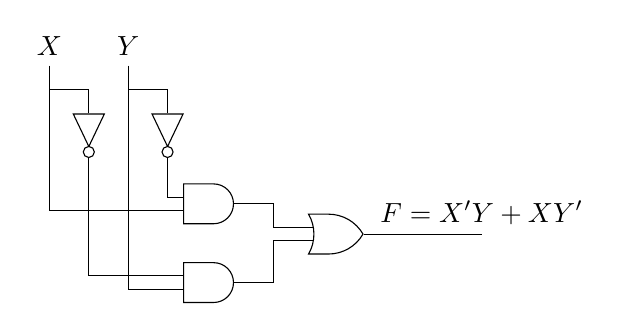
\begin{tikzpicture}[label distance=2mm]

    \node (X) at (0,0) {$X$};
    \node (Y) at (1,0) {$Y$};
     \node[not gate US, draw, rotate=-90] at ($(X)+(0.5,-1)$) (not1) {};
    \node[not gate US, draw, rotate=-90] at ($(Y)+(0.5,-1)$) (not2) {};
    \node[and gate US, draw, logic gate inputs=nn] at ($(X)+(2,-2)$) (and1) {};
    \node[and gate US, draw, logic gate inputs=nn] at ($(and1)+(0,-1)$) (and2) {};
    \node[or gate US, draw, logic gate inputs=nn, anchor=input 1] at ($(and1.output)+(1,-0.3)$) (or1) {};
    \draw (X) |- (and1.input 2);
    \draw (Y) |- (and2.input 2);
    \draw (not1) |- (and2.input 1);
    \draw (not2) |- (and1.input 1);
    \path (X) -- coordinate (punt)(X |- not1.input);
    \draw (punt)-| (not1.input);
    \path (Y) -- coordinate (punt)(Y |- not2.input);
    \draw (punt) -| (not2.input);
    \draw (and1.output) -- ([xshift=0.5cm]and1.output) |- (or1.input 1);
    \draw (and2.output) -- ([xshift=0.5cm]and2.output) |- (or1.input 2);
    \draw (or1.output) -- ([xshift=1.5cm]or1.output) node[above] {$F=X'Y +XY'$};
    \end{tikzpicture} 
\begin{center}
    Interal diagram of EX-OR gate.
\end{center}

 
 \section{Truth Table}
 The following is the truth table of EX-OR gate
\begin{table}[htbp]
 \begin{center}
    \begin{tabular}{|c|c|c|c|c|c|c|c|c|} \hline 
  \textbf{X}& \textbf{Y} &\textbf{F=X'Y+XY'} \\
 \hline
0&0&0\\ \hline
0&1&1 \\ \hline
1&0&1\\ \hline
1&1&0  \\ \hline
\end{tabular}   
\end{center}
\caption{\label{table:dummytable} }
\end{table}   
    
    
 
 \section{Components}
 
     \begin{tabularx}{0.4\textwidth} {  
  | >{\centering\arraybackslash}X  
  | >{\centering\arraybackslash}X  
  | >{\centering\arraybackslash}X |}
  \hline
\textbf{Component} &  \textbf{Value} & \textbf{Quantity}\\
\hline
Arduino & UNO & 1 \\  
\hline
Resistor& 220ohm & 1 \\ 
\hline
Bread board & - & 1 \\
\hline
Jumber wires & M-M & 20\\
\hline
LED & - & 1\\
\hline
\end{tabularx}

     
  \section{Hardware Connection}
  The inputs 'X' and 'Y' are read from the breadboard which are connected to pins '2','3' in Port D of Arduino and the ouput is take from the pin '5'of Arduino. The output is connected to LED. The respective connections are shown in the Table II.
	 \begin{table}[htbp]
 \begin{center}
    \begin{tabular}{|l|c|c|c|c|c|} \hline 
  \textbf{Arduino}& \textbf{2} & \textbf{3}&\textbf{5}\\
   \hline
 Inputs&X&Y&-\\ \hline
 Output&-&-&F\\ \hline
\end{tabular}   
\end{center}
\caption{\label{table:dummytable} }
\end{table}


	\section{Procedure}

1. Give the connections as per Table 2. For taking the inputs connect 5V of arduino to +ve line of bread board to consider it as logic 'HIGH',connect GND pin of arduino to -ve line of bread board to consider it as logic 'LOW'.
\\2. Since we know the output of EX-OR gate is '1', if and only if only one of the inputs is '1' and '0'in rest conditions. The same condition can be verified changing the inputs in breadboard.
\\3.Download the follwing code
\begin{lstlisting}
https://github.com/riyaziith/FWC-Module1
\end{lstlisting}
 4.Upload the code into the Arduino board using USB cable.
\\5.The output '1' is represented as the state:'LED ON' and '0' is represented as the state 'LED OFF'
\end{document}